\chapter[Alternative method for computing European compound options]{Alternative method for computing European compound options}
\chaptermark{European compound options}

\section{Outline}
This chapter will be outlined as follows. We will introduce the general compound options pricing formula in Section 6.2 with examples of application. This section also contains an interesting type of put-call parity that can occur for European vanilla compound options. In Section 6.3, we demonstrate the versatility of our pricing formula for a non-standard compound option. The variation to the pricing compound options when the underlying asset pays one discrete dividend is examined in Section 6.4. Closing remarks regarding these findings are provided in Section 6.5.

\section{Generalised compound option pricing formulas}
\label{sec:gen}
A compound option pricing formula for general payoffs will now be introduced. To begin, we first denote two options by $v_1$ and $v_2$ with payoffs $\phi_1$ and $\phi_2$ at expiry times $T_1$ and $T_2$, respectively. We also assume that $T_1 < T_2$. We now construct a compound option where $v_1$ has an underlying that is the second option $v_2$. We can express this mathematically from~\eqref{eqn:optionKernelSoln} to give
	\begin{equation}
		\label{eqn:v1aa}
		v_1(x,t) = \int_0^\infty \fr{1}{y}\K\left( \fr{x}{y}, t, T_1 \right)\phi_1(v_2(y,T_1)) \, \d y,
	\end{equation}
where
	\begin{equation}
		\label{eqn:v2a}
		v_2(y,T_1) = \int_0^\infty \fr{1}{z}\K\left( \fr{y}{z}, T_1, T_2 \right)\phi_2(z)\, \d z.
	\end{equation}
%With the aid of Corollary 1, it is possible to express all financial payoffs seen in options pricing and thus generate pricing formulas using~\eqref{eqn:v1aa} and~\eqref{eqn:v2a}.
We will illustrate how this works with the four standard European compound options.

\subsection{Call-on-a-call compound option}
A call-on-a-call option, denoted by $v_{\text{cc}}$, is composed of two European call options with two different strikes $K_1$ and $K_2$ and payoffs $\phi_1(x) = \max(x - K_1, 0)$ at $T_1$ and $\phi_2(x) = \max(x - K_2, 0)$ at $T_2$, respectively. Using \eqref{eqn:v1aa}, where we identify $v_1$ with $v_\mathrm{cc}$ and $v_2$ with $v_\mathrm{c}$, we obtain
	\begin{equation*}
		v_{\text{cc}}(x,t) = \int_0^\infty \fr{1}{y} \K\left( \fr{x}{y}, t, T_1 \right)\max(v_\text{c}(y,T_1; K_2, T_2) - K_1, 0)\, \d y.
	\end{equation*}
To proceed, we assume that $v_{\text{c}}(y,T_1; K_2, T_2) > K_1$ for all $y$ greater than some critical value $y_\mathrm{c}^*$~\cite{Kwok2008}. Due to the monotonicity of a European call with respect to the asset value, this critical value $y_\mathrm{c}^*$ will always be unique (see Figure~\ref{fig:1}). This simplifies the integral to
	\begin{align*}
		v_{\text{cc}}(x,t) &= \int_{y_\mathrm{c}^*}^\infty \fr{1}{y}\K\left( \fr{x}{y}, t, T_1 \right)[v_\text{c}(y,T_1; K_2, T_2) - K_1] \, \d y \\
		&= \int_{y_\mathrm{c}^*}^\infty \fr{1}{y} \K\left( \fr{x}{y}, t, T_1 \right)v_\text{c}(y,T_1; K_2, T_2) \, \d y - K_1\int_{y_\mathrm{c}^*}^\infty \fr{1}{y}\K\left( \fr{x}{y}, t, T_1 \right) \, \d y.
	\end{align*}

\begin{figure}[!h]
	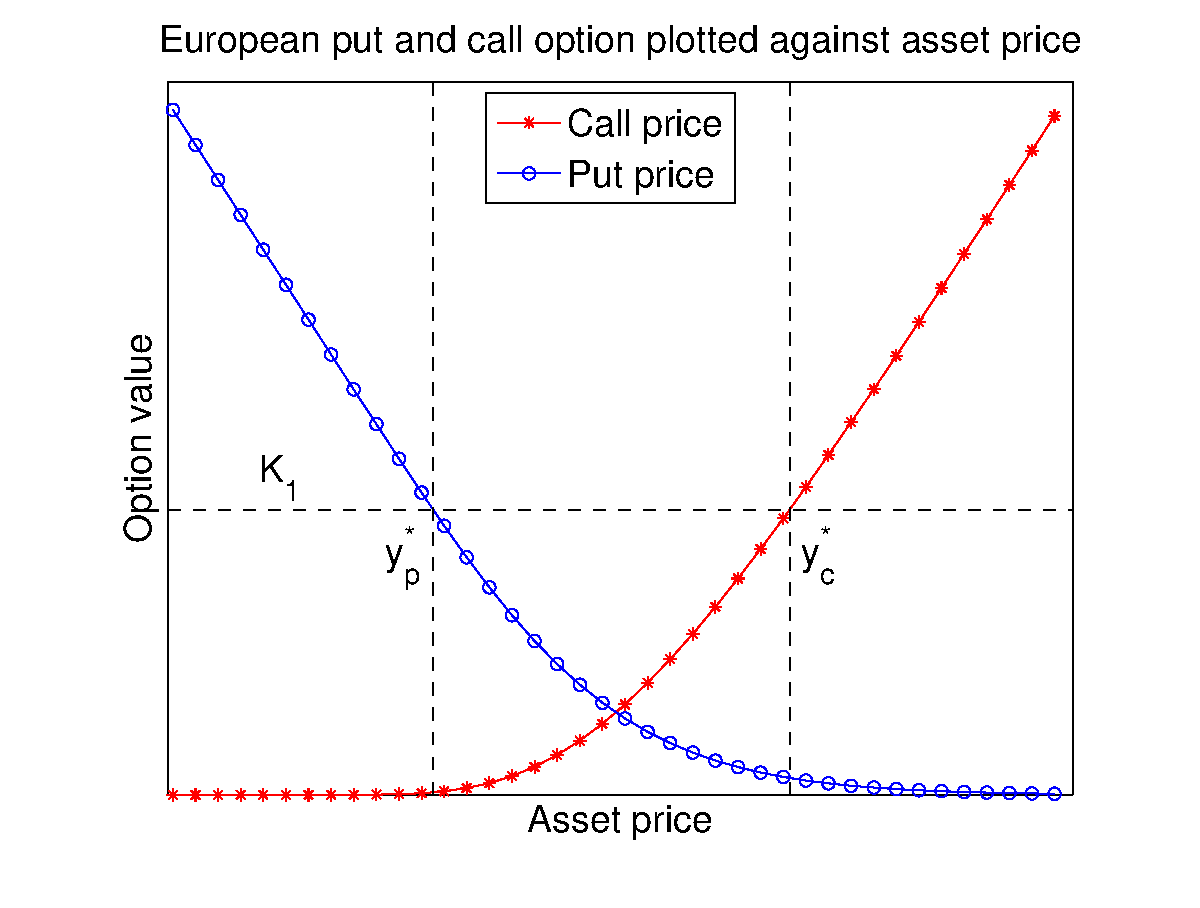
\includegraphics[scale=0.5]{figures/option.eps}
		\centering
		\caption{The European call~\eqref{eqn:EUcall} and European put~\eqref{eqn:EUput} plotted against $x$ for a fixed $t \in [0,T)$. The horizontal line that intersects both profiles is some strike price $K_1$ associated with the compound option. The intersection values correspond to the critical values ($y_\text{c}^*$ for a call and $y_\text{p}^*$ for a put) the underlying option must be below or above in order to have a positive payoff for the compound option.}
		\label{fig:1}
\end{figure}
\noindent
Using \eqref{eqn:optionKernelSoln} for $v_\text{c}$ gives
	\begin{align*}
		v_\text{cc}(x,t) &= \int_{y_\mathrm{c}^*}^\infty \fr{1}{y}\K\left( \fr{x}{y}, t, T_1 \right)\int_0^\infty \fr{1}{z} \K\left( \fr{y}{z}, T_1, T_2 \right)\max(z-K_2, 0) \, \d z \, \d y \\
		& \quad - K_1\int_{y_\mathrm{c}^*}^\infty \fr{1}{y}\K\left( \fr{x}{y}, t, T_1 \right) \, \d y \\
		&=  \int_{y_\mathrm{c}^*}^\infty \int_{K_2}^\infty \fr{1}{y}\K\left( \fr{x}{y}, t, T_1 \right)\K\left( \fr{y}{z}, T_1, T_2 \right) \, \d z \, \d y \\
		& \quad - K_2 \int_{y_\mathrm{c}^*}^\infty \int_{K_2}^\infty \fr{1}{y}\K\left( \fr{x}{y}, t, T_1 \right)\fr{1}{z}\K\left( \fr{y}{z}, T_1, T_2 \right) \, \d z \, \d y - K_1\int_{y_\mathrm{c}^*}^\infty \fr{1}{y}\K\left( \fr{x}{y}, t, T_1 \right) \, \d y.
	\end{align*}
We evaluate each integral using~\eqref{eqn:inta}\,--\,\eqref{eqn:int2} in Corollary 1 by choosing $a_1 = y_\mathrm{c}^*$, $b_1 = \infty$, $a_2 = K_2$, and $b_2 = \infty$. Using~\eqref{eqn:Nspecial}, we have
	\begin{equation}
		\label{eqn:vcc}
		\begin{split}
		v_\text{cc}(x,t) &=  xe^{-\int_t^{T_2} q(\tau) \, \d\tau}N_2\left( z_1\left( \fr{x}{y_\mathrm{c}^*}, t, T_1 \right), z_1\left( \fr{x}{K_2}, t, T_2 \right); \rho^* \right)  \\
		&\quad - K_2e^{-\int_t^{T_2} r(\tau) \, \d\tau} N_2\left( z_2\left( \fr{x}{y_\mathrm{c}^*}, t, T_1 \right), z_2\left( \fr{x}{K_2}, t, T_2 \right); \rho^* \right) \\
		&\quad - K_1e^{-\int_t^{T_1} r(\tau) \,\d\tau}N\left( z_2\left( \fr{x}{y_\mathrm{c}^*}, t, T_1 \right) \right),
		\end{split}
	\end{equation}
where
	\begin{equation}
		\label{eqn:rho2}
		\rho^* = \left(\fr{\int_t^{T_1} \sigma(\tau)^2 \, \d\tau}{\int_t^{T_2} \sigma(\tau)^2 \, \d\tau}\right)^{1/2}.
	\end{equation}
This agrees with the results derived by Geske~\cite{Geske1979} and Kwok~\cite{Kwok2008} who both implemented a probabilistic approach via a risk-neutral measure to compute the pricing formula.

\subsection{Put-on-a-put compound option}
In contrast to the call-on-a-call option, a put-on-a-put option $v_\mathrm{pp}$ comprises of a European put option with a strike $K_1$ and payoff $\phi_1(x) = \max(K_1-x,0)$ at $T_1$ with an underlying European put option with strike $K_2$ and payoff $\phi_2(x) = \max(K_2-x,0)$ at $T_2$. Using~\eqref{eqn:v1aa} where we identify $v_1$ with $v_\mathrm{pp}$ and $v_2$ with $v_\mathrm{p}$, we obtain
	$$
		v_\mathrm{pp}(x,t) = \int_0^\infty \fr{1}{y}\K\left( \fr{x}{y}, t, T_1 \right)\max(K_1 - v_\mathrm{p}(y,T_1;K_2,T_2), 0) \, \d y.
	$$
We want the values of $y$ such that $v_\mathrm{p}(y,T_1;K_2,T_2) < K_1$ to ensure a strictly positive argument for the payoff $\phi_1$. According to Figure~\ref{fig:1}, this corresponds to $y > y_\mathrm{p}^*$. Although the European put option profile also exhibits monotonic (decreasing) behaviour, there is an extra restriction for $y_\mathrm{p}^*$ to be unique. At $y=0$, the underlying put option will be
	$$
		v_\text{p}(0,T_1) = K_2e^{-\int_{T_1}^{T_2} r(\tau) \, \d\tau}.
	$$
	In order for $y_\text{p}^*$ to be unique, we require
	\begin{equation}
		\label{eqn:pprestriction}
		K_1 \leq K_2e^{-\int_{T_1}^{T_2} r(\tau) \, \d\tau},
	\end{equation}
	since the intersection of $K_1$ with the option profile will represent the critical value for the compound option. If $K_1 > K_2e^{-\int_{T_1}^{T_2} r(\tau) \, \d\tau}$, there will be no intersection with the European put option curve and thus no critical value for the compound option.

Substituting $v_\mathrm{p}$ for its integral expression using~\eqref{eqn:optionKernelSoln}, we have
	\begin{align*}
		v_\text{pp}(x,t) &= K_1\int_{y_\mathrm{p}^*}^\infty \fr{1}{y}\K\left( \fr{x}{y}, t, T_1 \right) \, \d y \\
		&\quad - \int_{y_\mathrm{p}^*}^\infty \fr{1}{y}\K\left( \fr{x}{y}, t, T_1 \right)\int_0^\infty \fr{1}{z} \K\left( \fr{y}{z}, T_1, T_2 \right)\max(K_2-z, 0) \, \d z \, \d y 		\\
		&=  K_1\int_{y_\mathrm{p}^*}^\infty \fr{1}{y}\K\left( \fr{x}{y}, t, T_1 \right) \, \d y - K_2 \int_{y_\mathrm{p}^*}^\infty \int_{0}^{K_2} \fr{1}{y}\K\left( \fr{x}{y}, t, T_1 \right)\fr{1}{z}\K\left( \fr{y}{z}, T_1, T_2 \right) \, \d z \, \d y \\
		&\quad +  \int_{y_\mathrm{p}^*}^\infty \int_{0}^{K_2} \fr{1}{y}\K\left( \fr{x}{y}, t, T_1 \right)\K\left( \fr{y}{z}, T_1, T_2 \right) \, \d z \, \d y.
	\end{align*}
Once again, each integral is evaluated using~\eqref{eqn:inta}\,--\,\eqref{eqn:int2} in Corollary 1 and simplified using~\eqref{eqn:Nspecial}. Choosing $a_1 = y_\mathrm{p}^*$, $b_1 = \infty$, $a_2 = 0$, and $b_2 = K_2$ yields
	\begin{align}
		v_\text{pp}(x,t) &=  K_2e^{-\int_t^{T_2} r(\tau) \, \d\tau}\left[ N_2\left( z_2\left( \fr{x}{y_\mathrm{p}^*}, t, T_1 \right), z_2\left( \fr{x}{K_2}, t, T_2 \right); \rho^* \right) - N\left(z_2\left( \fr{x}{y_\text{p}^*},t, T_1 \right)\right)\right] \nonumber \\ %\label{eqn:vpp}  \\ \\
		&\quad - xe^{-\int_t^{T_2} q(\tau) \, \d\tau}\left[ N_2\left( z_1\left( \fr{x}{y_\text{p}^*}, t, T_1 \right), z_1\left( \fr{x}{K_2}, t, T_2 \right); \rho^* \right) - N\left(z_1\left( \fr{x}{y_\text{p}^*},t, T_1 \right)\right)\right] \nonumber \\
		&\quad + K_1e^{-\int_t^{T_1} r(\tau) \,\d\tau}N\left( z_2\left( \fr{x}{y_\text{p}^*}, t, T_1 \right) \right), \nonumber
	\end{align}
where $\rho^*$ is the same as in~\eqref{eqn:rho2}.

\subsection{Call-on-a-put compound option}
We will use~$v_\mathrm{cp}$ for the value of a call-on-a-put compound option. This is made up of a European call option with a strike price $K_1$ and payoff $\phi_1(x) = \max(x-K_1,0)$ at $T_1$ with an underlying European put option with strike $K_2$ and payoff $\phi_2(x) = \max(K_2-x,0)$ at $T_2$.  From~\eqref{eqn:v1aa}, we associate $v_1$ with $v_\mathrm{cp}$ and $v_2$ with $v_\mathrm{p}$ to get
	$$
		v_\mathrm{cp}(x,t) = \int_0^\infty \fr{1}{y}\K\left( \fr{x}{y}, t, T_1 \right)\max(v_\mathrm{p}(y,T_1;K_2,T_2) - K_1, 0) \, \d y.
	$$
We assume the $v_\mathrm{p}(y,T_1;K_2,T_1) > K_1$ to ensure that the payoff $\phi_1$ is positive. However in contrast to the previous examples, we need to be \emph{below} the critical value $y_\text{p}^*$ (since the underlying is a put option) in order to achieve this (see Figure~\ref{fig:1}). We also express $v_\text{p}$ in integral form using~\eqref{eqn:optionKernelSoln} which leaves us with
		\begin{align*}
		v_\text{cp}(x,t) &= \int_{0}^{y_\mathrm{p}^*} \fr{1}{y}\K\left( \fr{x}{y}, t, T_1 \right)\int_0^\infty \fr{1}{z} \K\left( \fr{y}{z}, T_1, T_2 \right)\max(K_2-z, 0) \, \d z \, \d y \\
		& \quad - K_1\int_{0}^{y_\mathrm{p}^*} \fr{1}{y}\K\left( \fr{x}{y}, t, T_1 \right) \, \d y \\
		&=  K_2\int_{0}^{y_\mathrm{p}^*} \int_{0}^{K_2} \fr{1}{y}\K\left( \fr{x}{y}, t, T_1 \right)\fr{1}{z}\K\left( \fr{y}{z}, T_1, T_2 \right) \, \d z \, \d y \\
		& \quad - \int_{0}^{y_\mathrm{p}^*} \int_0^{K_2} \fr{1}{y}\K\left( \fr{x}{y}, t, T_1 \right)\K\left( \fr{y}{z}, T_1, T_2 \right) \, \d z \, \d y - K_1\int_{0}^{y_\mathrm{p}^*} \fr{1}{y}\K\left( \fr{x}{y}, t, T_1 \right) \, \d y,
	\end{align*}
where we still assume~\eqref{eqn:pprestriction} to ensure uniqueness for $y_\text{p}^*$. Using Corollary 1 with $a_1 = 0$, $b_1 = y_\mathrm{p}^*$, $a_2 = 0$, and $b_2 = K_2$ and upon simplifying all the $N$ and $N_2$ terms using~\eqref{eqn:Nspecial}, we get	\begin{equation}
		\label{eqn:vcp}
		\begin{split}
		v_\text{cp}(x,t) &= v_\text{pp}(x,t) + v_\text{p}(x,t;K_2,T_2) - K_1e^{-\int_t^{T_1} r(\tau) \, \d\tau}.
		\end{split}
	\end{equation}
Eq.~\eqref{eqn:vcp} behaves like a pseudo-put-call parity between $v_\text{pp}$ and $v_\text{cp}$. It should be highlighted that this equation bares a strong similarity to the standard put-call parity result~\eqref{eqn:pcp}. We will witness a similar occurrence for a put-on-a-call compound option next.
	
\subsection{Put-on-a-call compound option}
The final standard combination is a put-on-a-call compound option, which we will label $v_\text{pc}$. This option is constructed with a European put option with strike $K_1$ and payoff $\phi_1(x) = \max(K_1-x,0)$ at $T_1$ with an underlying European call option with strike $K_2$ and payoff $\phi_2(x) = \max(x-K_2,0)$ at $T_2$. Setting $v_1$ to $v_\text{pc}$ and $v_2$ to $v_\text{c}$ in~\eqref{eqn:v1aa} results in

\begin{equation*}
		v_{\text{pc}}(x,t) = \int_0^\infty \fr{1}{y} \K\left( \fr{x}{y}, t, T_1 \right)\max(K_1 -v_\text{c}(y,T_1; K_2, T_2), 0)\, \d y.
	\end{equation*}
For $v_{\text{c}}(y,T_1; K_2, T_2) < K_1$ to be satisfied and guarantee a positive payoff $\phi_1$, we need to be below $y_\text{c}^*$ according to Figure~\ref{fig:1} (since the option being compounded on is a European call). This simplifies  to
	\begin{align*}
		v_\text{pc}(x,t) &= K_1\int_{0}^{y_\mathrm{c}^*} \fr{1}{y}\K\left( \fr{x}{y}, t, T_1 \right) \, \d y - \int_{0}^{y_\mathrm{c}^*} \fr{1}{y} \K\left( \fr{x}{y}, t, T_1 \right)v_\text{c}(y,T_1; K_2, T_2) \, \d y.
	\end{align*}
Once again incorporating \eqref{eqn:optionKernelSoln} for $v_\text{c}$ leads to
	\begin{align*}
		v_\text{pc}(x,t) &= K_1\int_{0}^{y_\mathrm{c}^*} \fr{1}{y}\K\left( \fr{x}{y}, t, T_1 \right) \, \d y \\
		&\quad - \int_0^{y_\mathrm{c}^*}\fr{1}{y}\K\left( \fr{x}{y}, t, T_1 \right)\int_0^\infty \fr{1}{z} \K\left( \fr{y}{z}, T_1, T_2 \right)\max(z-K_2,0) \, \d z \, \d y \\
		&= K_1\int_{0}^{y_\mathrm{c}^*} \fr{1}{y}\K\left( \fr{x}{y}, t, T_1 \right) \, \d y - \int_0^{y_\mathrm{c}^*}\int_{K_2}^\infty \fr{1}{y}\K\left( \fr{x}{y},t,T_1 \right)\K\left( \fr{y}{z}, T_1, T_2 \right) \, \d z \, \d y \\
		&\quad + K_2\int_0^{y_\mathrm{c}^*}\int_{K_2}^\infty\fr{1}{y}\K\left( \fr{x}{y}, t, T_1 \right) \fr{1}{z} \K\left( \fr{y}{z}, T_1, T_2 \right) \d z \, \d y .
	\end{align*}
Choosing $a_1 = 0$, $b_1 = y_\mathrm{c}^*$, $a_2 = K_2$, and $b_2 = \infty$ for Corollary 1 will give
\begin{equation}
		\label{eqn:vpc}
		\begin{split}
		v_\text{pc}(x,t) &= v_\text{cc}(x,t) - v_\text{c}(x,t;K_2,T_2) + K_1e^{-\int_t^{T_1} r(\tau) \, \d\tau},
		\end{split}
	\end{equation}
where $\rho^*$ is as in~\eqref{eqn:rho2} and~\eqref{eqn:Nspecial} was used to simplify the $N$ and $N_2$ terms. This is the pseudo-put-call parity relation between $v_\text{cc}$ and $v_\text{pc}$. It should be stressed the critical values $y_\text{c}^*$ and $y_\text{p}^*$ may not necessarily be equal, thus a put-call parity relating $v_\text{cc}$ and $v_\text{pp}$ without a dependence on $v_\text{pc}$ and $v_\text{cp}$ is unlikely to be ascertained unless in special circumstances (e.g., $y_\text{c}^* = y_\text{p}^*$). However, adding~\eqref{eqn:vcp} to~\eqref{eqn:vpc} and rearranging gives us
	\begin{equation*}
		v_\text{cc}(x,t) + v_\text{pp}(x,t) = v_\text{pc}(x,t) + v_\text{cp}(x,t) + v_\text{c}(x,t; K_2, T_2) - v_\text{p}(x,t; K_2, T_2)
	\end{equation*}
Now using~\eqref{eqn:pcp}, we can relate $v_\text{c}(x,t; K_2, T_2)$ to $v_\text{p}(x,t; K_2, T_2)$ and obtain
	\begin{equation}
		\label{eqn:pseudopcp}
		v_\text{cc}(x,t) + v_\text{pp}(x,t) =  v_\text{pc}(x,t) + v_\text{cp}(x,t) + xe^{-\int_t^{T_2} q(\tau) \, \d\tau} - K_2e^{-\int_t^{T_2} r(\tau) \, \d\tau},
	\end{equation}
which resembles the standard put-call parity identity in~\eqref{eqn:pcp} in form. Another interesting route would have been to incorporate a portfolio argument to arrive at~\eqref{eqn:pseudopcp}, but we opted for our presented approach as it ties in closely with the results from this work.

\section{Generalised example: straddle-on-a-call compound option}
We outlined in Section~\ref{sec:gen} that the results in Corollary 1 can be implemented for any financial payoff in options pricing to generate any compound option pricing formula. This is attainable since any of the aforementioned payoffs can be expressed as finite linear combinations of the functions
	\begin{equation}
		\label{eqn:funcs}
		x \mapsto \1_I(x), \quad x \mapsto x\1_I(x),
	\end{equation}
where $\1_I$ is the indicator function defined as
	\begin{equation*}
		\1_I(x) = \begin{cases}
			1, \quad x \in I, \\
			0, \quad x \notin I,
		\end{cases}
	\end{equation*}
and where $I$ is an arbitrary interval with endpoints $a$ and $b$ with $a < b$. The interval can be open, half-closed, or closed. \textcolor{blue}{The two auxiliary functions in~\eqref{eqn:funcs} are the building blocks for many financial payoffs in options pricing.} For example, a call option has a payoff $\max(x-K,0)$ which can be written as
	\begin{equation*}
		\max(x-K,0) = x\1_{[K,\infty)}(x) - K\1_{[K,\infty)}(x),
	\end{equation*}
where the interval $I$ is $[K,\infty)$.

In general, there are four possibilities for the auxiliary functions to consider in compound options:
	\begin{enumerate}
		\item $\phi_1(x) = \1_I(x)$, $\phi_2(x) = \1_I(x)$,
		\item $\phi_1(x) = \1_I(x)$, $\phi_2(x) = x\1_I(x)$,
		\item $\phi_1(x) = x\1_I(x)$, $\phi_2(x) = \1_I(x)$,
		\item $\phi_1(x) = x\1_I(x)$, $\phi_2(x) = x\1_I(x)$.
	\end{enumerate}
Using~\eqref{eqn:v1aa} and~\eqref{eqn:v2a}, it can be shown that the first two cases when used will result in~\eqref{eqn:inta} upon evaluation; \eqref{eqn:int1} will be the result when using the third case; and computation using the fourth possibility will yield \eqref{eqn:int2}. To highlight the flexibility and generality of~\eqref{eqn:funcs}, we will look at pricing a straddle-on-a-call option.

To set this up, we require two options: an outer straddle option with payoff $\max(x-K_1,0) + \max(K_1-x,0)$ at $t = T_1$, and an inner call option with payoff $\max(x-K_2,0)$ at $t = T_2$. We will denote a straddle by $v_{\text{s}}$ and the compound option by $v_{\text{sc}}$. So we have
	\begin{align*}
		v_\text{sc}(x,t) &= \int_0^\infty \fr{1}{y}\K\left( \fr{x}{y}, t, T_1 \right)\left[\max(v_\text{c}(y,T_1) - K_1, 0) + \max(K_1 - v_\text{c}(y,T_1), 0) \right] \, \d y.
	\end{align*}
Upon splitting up the terms, we notice we have the two integrals that formulate a call-on-a-call compound option and a put-on-a-call compound option, respectively. Thus,
	\begin{equation}
		\label{eqn:vsc}
			v_\text{sc}(x,t) = v_\text{cc}(x,t) + v_\text{pc}(x,t).
	\end{equation}
	
\section{Compound options with discrete dividends}
Up until now, the model we have presented for pricing compound options assumes a continuous dividend yield for the lifetime of the options. That is, $q$ is a time-continuous function. Here we introduce a technique to formulate compound options when the underlying asset pays one dividend yield at a fixed time. What we will show is that it is only one slight variation needed to the methodology used to derive all the previous formulas.

The underlying asset with a potential dividend yield (whether discrete or continuous) is governed by~\cite{Wilmott1995}
	\begin{equation*}
		%\label{eqn:SDE2}
		\d S_t = [r(t)S_t - D(S_t,t)] \, \d t + \sigma(t) S_t  \, \d W_t,
	\end{equation*}
where $D(S_t,t)$ does not necessarily to have be linear in $S_t$. It follows that a European option whose underlying follows the SDE above satisfies
	\begin{equation*}
		\fr{\pr v}{\pr t} + \fr{1}{2}\sigma(t)^2x^2\fr{\pr^2 v}{\pr x^2} + [r(t)x - D(x,t)]\fr{\pr v}{\pr x} - r(t)v = 0.
	\end{equation*}
This is a potential unified approach to pricing options regardless of whether the dividend yield is continuous or discrete. However, the Black-Scholes kernel identities in the preliminaries rely on the dividend term $D$ being linear in $x$ (i.e., $D(x,t) = q(t)x$). Therefore, in order to adapt the kernel identities, we have assumed a specific form for $D$ to be able to construct a pricing formula for discrete dividends.

To proceed, we assume a dividend of value proportional to the asset price is paid out on a date $t = t_d$, where $t_d$ is before the expiry. Consequently, this means that the asset price $S_t$ will decrease by a proportion of its value as it passes $t_d$. We call the proportion factor $q_d \in [0,1)$. Using $t_d^-$ and $t_d^+$ to indicate an infinitesimal time before and after the dividend payment date, respectively, mathematically this implies the following jump condition
	\begin{equation}
		\label{eqn:jumpcond}
		S_{t_d^+} = S_{t_d^-} - q_dS_{t_d^-} = (1-q_d)S_{t_d^-}.
	\end{equation}
A common way to price options when the underlying pays a discrete dividend is to solve the Black-Scholes equation~\eqref{eqn:blackscholes} backwards in time twice; once from expiry $T$ to $t_d^+$ and then from $t_d^-$ to an arbitrary time $t$~\cite{Wilmott1995, Jiang2005}. However, an extra step is required whereby the jump condition~\eqref{eqn:jumpcond} for $S_t$ needs to be accounted for as a boundary condition between $t_d^+$ and $t_d^-$.

We will first illustrate this concept of discrete dividend payments in a standard European option with payoff $\phi$. Suppose one dividend is paid at time $t_d \in (0,T)$. Once again, we denote $t_d^-$ and $t_d^+$ to be the moment before and after the dividend payment is made, respectively. Working backwards from $T$ to $t_d^+$, we define a function $w$ to be
		$$
			w(x,t) = \int_0^\infty \fr{1}{y} \K\left( \fr{x}{y},t, T \right)\phi(y) \, \d y, \quad t_d^+ \leq t \leq T,
		$$
where we used~\eqref{eqn:optionKernelSoln}. From the jump condition~\eqref{eqn:jumpcond}, we have
		$$
			w\left(S_{t_d^-},t_d^-\right) = w\left(S_{t_d^+},t_d^+\right) = w\left((1-q_d)S_{t_d^-},t_d^+\right).
		$$
This expression acts as our payoff from $t_d^-$ backwards to time-zero since it is the matching condition between $t_d^+$ and $t_d^-$. Therefore,
		\begin{equation}
			\label{eqn:cool}
			v(x,t) =
			\begin{cases}
				\ds\int_0^\infty \fr{1}{y} \K\left( \fr{x}{y}, t, t_d^- \right)w\left( (1-q_d)y, t_d^+ \right) \, \d y & \text{if } 0 \leq t \leq t_d^-, \\
				\ds\int_0^\infty \fr{1}{y} \K\left( \fr{x}{y}, t, T \right) \phi(y) \, \d y = w(x,t) & \text{if } t_d^+ \leq t \leq T.
			\end{cases}
		\end{equation}
For compound options paying only one discrete dividend, we have three cases to consider since we have two terminal dates $T_1$ and $T_2$ ($T_1 < T_2$) for the compound and underlying option, respectively. We assume that $0 < t_d < T_2$.

\subsection{Case 1: $0 < t_d < T_1 < T_2$}
In this scenario, we assume that the dividend payment is before the terminal date of the compound option (see Figure~\ref{fig:2}).

\begin{figure}[!h]
\centering
\begin{tikzpicture}
\draw (0,0) -- (8,0);
\draw (0pt,8pt) -- (0pt,-8pt) node[below,fill=white] {0};
\draw[xshift=1cm] (0pt,4pt) -- (0pt,-4pt) node[below,fill=white] {$t_d^-$};
\draw[xshift=2cm] (0pt,4pt) -- (0pt,-4pt) node[below,fill=white] {$t_d$};
\draw[xshift=3cm] (0pt,4pt) -- (0pt,-4pt) node[below,fill=white] {$t_d^+$};
\draw[xshift=4cm] (0pt,8pt) -- (0pt,-8pt) node[below,fill=white] {$T_1$};
\draw[xshift=8cm] (0pt,8pt) -- (0pt,-8pt) node[below,fill=white] {$T_2$};
\end{tikzpicture}
\caption{The dividend is paid on the date $t_d$ which is before the expiry $T_1$ of the compound option.}
\label{fig:2}
\end{figure}
\noindent
Working backwards from $T_1$ to $t_d^+$, we first define $w_1$ to be
		\begin{equation}
			\label{eqn:w1}
			w_1(x,t) = \int_0^\infty \fr{1}{y} \K\left( \fr{x}{y}, t, T_1 \right) \phi_1(v_2(y,T_1)) \, \d y, \quad t_d^+ \leq t \leq T_1,
		\end{equation}
where
		\begin{equation}
			\label{eqn:v2}
			v_2(y,T_1) = \int_0^\infty \fr{1}{z} \K\left( \fr{y}{z}, T_1, T_2 \right) \phi_2(z) \, \d z.
		\end{equation}
Equation~\eqref{eqn:w1} is valid since between $t_d^+$ and $T_1$, the compound option has not yet expired. Using~\eqref{eqn:jumpcond} to match across the boundary $t_d^+$ gives
		$$
			w_1\left(S_{t_d^-},t_d^-\right) = w_1\left(S_{t_d^+},t_d^+\right) = w_1\left((1-q_d)S_{t_d^-},t_d^+\right).
		$$
	Then for $0 \leq t \leq t_d^-$, we have
		$$
			v_1(x,t) = \int_0^\infty \fr{1}{y}\K\left( \fr{x}{y}, t, t_d^- \right)w_1\left((1-q_d)y, t_d^+\right) \, \d y.
		$$
	Thus the compound option $v_1$ is given by
		\begin{equation}
			\label{eqn:v1}
			v_1(x,t) =
			\begin{cases}
				\ds\int_0^\infty \fr{1}{y} \K\left( \fr{x}{y}, t, t_d^- \right)w_1\left( (1-q_d)y, t_d^+ \right) \, \d y & \text{if } 0 \leq t \leq t_d^-, \\
				\ds\int_0^\infty \fr{1}{y} \K\left( \fr{x}{y}, t, T_1 \right) \phi_1(v_2(y,T_1)) \, \d y & \text{if } t_d^+ \leq t \leq T_1,
			\end{cases}
		\end{equation}
	with $v_2$ defined as in \eqref{eqn:v2}.
In this case, the compound option needs to be ``segmented'' in a piecewise manner since the dividend payment date $t_d$ is situated before $T_1$ (i.e., during the compound option's lifespan). We will see in the next scenario how the location of $t_d$ changes the formula for a compound option under one discrete dividend payment.
	
\subsection{Case 2: $0 < T_1 < t_d < T_2$}
We also consider the circumstance where the dividend payment happens after the compound option has expired but before the expiry date of the underlying option it acts upon (see Figure~\ref{fig:3}).

\begin{figure}[!h]
\centering
\begin{tikzpicture}
\draw (0,0) -- (8,0);
\draw (0pt,8pt) -- (0pt,-8pt) node[below,fill=white] {0};
\draw[xshift=4cm] (0pt,8pt) -- (0pt,-8pt) node[below,fill=white] {$T_1$};
\draw[xshift=5cm] (0pt,4pt) -- (0pt,-4pt) node[below,fill=white] {$t_d^-$};
\draw[xshift=6cm] (0pt,4pt) -- (0pt,-4pt) node[below,fill=white] {$t_d$};
\draw[xshift=7cm] (0pt,4pt) -- (0pt,-4pt) node[below,fill=white] {$t_d^+$};
\draw[xshift=8cm] (0pt,8pt) -- (0pt,-8pt) node[below,fill=white] {$T_2$};
\end{tikzpicture}
\caption{The dividend is paid on the date $t_d$ after $T_1$, which is past the lifetime of the compound option but still before the expiry of the underlying option.}
\label{fig:3}
\end{figure}
\noindent
In this formulation, the underlying option will need to be expressed piecewise in contrast to the piecewise compound option~\eqref{eqn:v1}. Once again working backwards from $T_2$ to $t_d^+$, we define $w_2$ to be
		$$
			w_2(x,t) = \int_0^\infty \fr{1}{y}\K\left( \fr{x}{y}, t, T_2 \right)\phi_2(y) \, \d y, \quad t_d^+ \leq t \leq T_2.
		$$
The jump condition~\eqref{eqn:jumpcond} gives
		$$
			w_2\left(S_{t_d^-},t_d^-\right) = w_2\left(S_{t_d^+},t_d^+\right) = w_2\left((1-q_d)S_{t_d^-},t_d^+\right).
		$$
Then for $T_1 \leq t \leq t_d^-$, we have
		$$
			v_2(x,t) = \int_0^\infty \fr{1}{y} \K\left( \fr{x}{y}, t, t_d^- \right)w_2\left( (1-q_d)y, t_d^+ \right) \, \d y.
		$$
Therefore $v_2$ is given by
		\begin{equation}
			v_2(x,t) =
			\begin{cases}
				\ds\int_0^\infty \fr{1}{y} \K\left( \fr{x}{y}, t, t_d^- \right)w_2\left( (1-q_d)y, t_d^+ \right) \, \d y & \text{if } T_1 \leq t \leq t_d^-, \\
				\ds\int_0^\infty \fr{1}{y} \K\left( \fr{x}{y}, t, T_2 \right) \phi_2(y) \, \d y = w_2(x,t) & \text{if } t_d^+ \leq t \leq T_2.
			\end{cases}
		\end{equation}
Now for $0 \leq t \leq T_1$, the compound option $v_1$ will be
		\begin{equation}
			\label{eqn:v1a}
			v_1(x,t) = \int_0^\infty \fr{1}{y} \K\left( \fr{x}{y}, t, T_1 \right)\phi_1(v_2(y,T_1))\, \d y.
		\end{equation}

\subsection{Case 3: $0 < t_d = T_1 < T_2$}
The last possible case is when the dividend payment is issued on the expiry date of the compound option (see Figure~\ref{fig:4}). As we will see, this unfolds to be quite an easy solution.

\begin{figure}[!h]
\centering
\begin{tikzpicture}
\draw (0,0) -- (8,0);
\draw (0pt,8pt) -- (0pt,-8pt) node[below,fill=white] {0};
\draw[xshift=3cm] (0pt,4pt) -- (0pt,-4pt) node[below,fill=white] {$t_d^-$};
\draw[xshift=4cm] (0pt,8pt) -- (0pt,-8pt) node[below,fill=white] {$t_d = T_1$};
\draw[xshift=5cm] (0pt,4pt) -- (0pt,-4pt) node[below,fill=white] {$t_d^+$};
\draw[xshift=8cm] (0pt,8pt) -- (0pt,-8pt) node[below,fill=white] {$T_2$};
\end{tikzpicture}
\caption{The dividend is paid on the date the compound option expires, which implies that $t_d = T_1$.}
\label{fig:4}
\end{figure}
\noindent
Working backwards from $T_2$ to $t_d^+$, we have
		\begin{equation}
			\label{eqn:v2b}
			v_2(x,t) = \int_0^\infty \fr{1}{z} \K\left( \fr{x}{z}, t, T_2 \right) \phi_2(y) \, \d y, \quad t_d^+ \leq t \leq T_2.
		\end{equation}
Using~\eqref{eqn:jumpcond} to match the boundaries, we get
		$$
			v_2\left(S_{t_d^-},t_d^-\right) = v_2\left(S_{t_d^+},t_d^+\right) = v_2\left((1-q_d)S_{t_d^-},t_d^+\right),
		$$
which gives us
		\begin{equation}
			\label{eqn:v1c}
			v_1(x,t) = \int_0^\infty \fr{1}{y} \K\left( \fr{x}{y}, t, t_d^- \right) v_2((1-q_d)y, t_d^+) \, \d y, \quad 0 \leq t \leq t_d^-.
		\end{equation}

\subsection{Example: Call-on-a-call for $0 < t_d < T_1 < T_2$}
We will now demonstrate how to apply one of the aforementioned general formulas in a discrete dividend setting to a European call-on-a-call compound option assuming Case 1. Using~\eqref{eqn:v1}, for $t_d^+ \leq t \leq T_1$, we just have a standard call-on-a-call since the dividend has been paid. We define a function $w_\text{cc}$ to represent this and it gives
	\begin{equation*}
		\begin{split}
		w_\text{cc}(x,t) &=  \int_{y_\mathrm{c}^*}^\infty \int_{K_2}^\infty \fr{1}{y}\K\left( \fr{x}{y}, t, T_1 \right)\K\left( \fr{y}{z}, T_1, T_2 \right) \, \d z \, \d y \\
		& \quad - K_2 \int_{y_\mathrm{c}^*}^\infty \int_{K_2}^\infty \fr{1}{y}\K\left( \fr{x}{y}, t, T_1 \right)\fr{1}{z}\K\left( \fr{y}{z}, T_1, T_2 \right) \, \d z \, \d y - K_1\int_{y_\mathrm{c}^*}^\infty \fr{1}{y}\K\left( \fr{x}{y}, t, T_1 \right) \, \d y,
	\end{split}
	\end{equation*}
recalling the integral expression before~\eqref{eqn:vcc}, where $y_\mathrm{c}^*$ is the associated critical value and $\rho^*$ is defined in~\eqref{eqn:rho2}. For notational simplicity, we define $\alpha = 1-q_d$. Then for $0 \leq t \leq t_d^-$, we use the first part of~\eqref{eqn:v1} to get
		\begin{equation*}
			\begin{split}
				v_\text{cc}(x,t) &= \int_0^\infty \fr{1}{y}\K\left( \fr{x}{y}, t, t_d^- \right)w_\text{cc}\left( \alpha y, t_d^+ \right) \, \d y \\
				&= \int_0^\infty \int_{y_\mathrm{c}^*}^\infty \int_{K_2}^\infty \fr{1}{y}\K\left( \fr{x}{y}, t, t_d^- \right) \fr{1}{z}\K\left( \fr{\alpha y}{z}, t_d^+, T_1 \right)\K\left( \fr{z}{w}, T_1, T_2 \right) \, \d w \, \d z \, \d y \\
				&\quad - K_2\int_0^\infty \int_{y_\mathrm{c}^*}^\infty \int_{K_2}^\infty \fr{1}{y}\K\left( \fr{x}{y}, t, t_d^- \right) \fr{1}{z}\K\left( \fr{\alpha y}{z}, t_d^+, T_1 \right)\fr{1}{w}\K\left( \fr{z}{w}, T_1, T_2 \right) \, \d w \, \d z \, \d y \\
				&\quad - K_1\int_0^\infty \int_{y_\mathrm{c}^*}^\infty \fr{1}{y}\K\left( \fr{x}{y}, t, t_d^- \right) \fr{1}{z}\K\left( \fr{\alpha y}{z}, t_d^+, T_1 \right) \, \d z \, \d y \\
				&= I_1 + I_2 + I_3.
			\end{split}
		\end{equation*}
Looking at $I_1$, the triple integral is in fact iterated. Therefore we arrange the order of integration with respect to $y$ first, then
		\begin{align*}
			I_1 &=  \int_{y_\mathrm{c}^*}^\infty \int_{K_2}^\infty \fr{1}{z} \K\left( \fr{z}{w}, T_1, T_2 \right)\int_0^\infty \fr{1}{y}\K\left( \fr{x}{y}, t, t_d^- \right) \K\left( \fr{\alpha y}{z}, t_d^+, T_1 \right) \, \d y \, \d w \, \d z \\
			& =\int_{y_\mathrm{c}^*}^\infty \int_{K_2}^\infty \fr{1}{z} \K\left( \fr{z}{w}, T_1, T_2 \right)\K_d\left( \fr{\alpha x}{z}, t, t_d^-, t_d^+, T_1 \right) \,  \d w \, \d z,
		\end{align*}
where~\eqref{eqn:intlem1} was implemented to simplify the innermost integral. Now using~\eqref{eqn:cor2c} in conjunction with~\eqref{eqn:Nspecial}, we obtain
	$$
		I_1 = \alpha xe^{-\int_t^{t_d^-} q(\tau) \, \d\tau - \int_{t_d^+}^{T_2} q(\tau)\,\d\tau}N_2\left( y_1\left( \fr{\alpha x}{y_\text{c}^*}, t, t_d^-, t_d^+, T_1 \right), y_1\left( \fr{\alpha x}{K_2}, t, t_d^-, t_d^+, T_2 \right); \rho_d^* \right),
	$$
where
	$$
		\rho_d^* = \left[ \fr{\int_t^{t_d^-} \sigma(\tau)^2 \,\d\tau + \int_{t_d^+}^{T_1} \sigma(\tau)^2 \, \d\tau}{\int_t^{t_d^-} \sigma(\tau)^2 \,\d\tau + \int_{t_d^+}^{T_2} \sigma(\tau)^2 \,\d\tau} \right].
	$$
For $I_2$, we do a similar process but incorporate~\eqref{eqn:cor2b} with~\eqref{eqn:Nspecial} to give
	\begin{align*}
		 I_2 &=  -K_2\int_{y_\mathrm{c}^*}^\infty \int_{K_2}^\infty \fr{1}{zw} \K\left( \fr{z}{w}, T_1, T_2 \right)\int_0^\infty \fr{1}{y}\K\left( \fr{x}{y}, t, t_d^- \right) \K\left( \fr{\alpha y}{z}, t_d^+, T_1 \right) \, \d y \, \d w \, \d z \\
			& =-K_2\int_{y_\mathrm{c}^*}^\infty \int_{K_2}^\infty \fr{1}{w} \K\left( \fr{z}{w}, T_1, T_2 \right)\fr{1}{z}\K_d\left( \fr{\alpha x}{z}, t, t_d^-, t_d^+, T_1 \right) \,  \d w \, \d z \\
			&= -K_2e^{-\int_t^{t_d^-} r(\tau) \, \d\tau - \int_{t_d^+}^{T_2} r(\tau)\,\d\tau}N_2\left( y_2\left( \fr{\alpha x}{y_\text{c}^*}, t, t_d^-, t_d^+, T_1 \right), y_2\left( \fr{\alpha x}{K_2}, t, t_d^-, t_d^+, T_2 \right); \rho_d^* \right).
	\end{align*}
Lastly for $I_3$, we swap the order of integration and use~\eqref{eqn:cor2a} with~\eqref{eqn:Nspecial} to yield
	\begin{align*}
		I_3 = -K_1e^{-\int_t^{t_d^-} r(\tau) \, \d\tau - \int_{t_d^+}^{T_1} r(\tau)\,\d\tau}N\left( y_2\left( \fr{\alpha x}{y_\text{c}^*}, t, t_d^-, t_d^+, T_1 \right) \right).
	\end{align*}
Putting this together, we arrive at the European call-on-a-call compound option for when the underlying asset pays a discrete dividend:
	\begin{equation}
	\label{eqn:vccd}
	\begin{split}
		v_\text{cc} &= \alpha xe^{-\int_t^{t_d^-} q(\tau) \, \d\tau - \int_{t_d^+}^{T_2} q(\tau)\,\d\tau}N_2\left( y_1\left( \fr{\alpha x}{y_\text{c}^*}, t, t_d^-, t_d^+, T_1 \right), y_1\left( \fr{\alpha x}{K_2}, t, t_d^-, t_d^+, T_2 \right); \rho_d^* \right) \\
		& \quad -K_2e^{-\int_t^{t_d^-} r(\tau) \, \d\tau - \int_{t_d^+}^{T_2} r(\tau)\,\d\tau}N_2\left( y_2\left( \fr{\alpha x}{y_\text{c}^*}, t, t_d^-, t_d^+, T_1 \right), y_2\left( \fr{\alpha x}{K_2}, t, t_d^-, t_d^+, T_2 \right); \rho_d^* \right) \\
		& \quad -K_1e^{-\int_t^{t_d^-} r(\tau) \, \d\tau - \int_{t_d^+}^{T_1} r(\tau)\,\d\tau}N\left( y_2\left( \fr{\alpha x}{y_\text{c}^*}, t, t_d^-, t_d^+, T_1 \right) \right).
	\end{split}
	\end{equation}
It should be highlighted that~\eqref{eqn:vccd} is identical in form to~\eqref{eqn:vcc} except the accompanying coefficients (e.g., $\alpha x$ instead of just $x$) have different arguments inside the $N_2$ to represent the discrete dividend payment. Note that when there is no discrete dividend payment (i.e., $q_d = 0$), we get $\alpha = 1$ and~\eqref{eqn:vccd} recovers~\eqref{eqn:vcc}.

	

%The method we establish does not require any extraneous steps and jump condition is completely accounted for.

%To capture this behaviour of a discrete dividends into the Black-Scholes framework, we set
%	\begin{equation}
%		\label{eqn:discrete}
%		D(x,t) = q\delta(t-t_d)x,
%	\end{equation}
%where $\delta$ is the standard Dirac delta function. Thus, the dynamics of the asset price process becomes
%	$$
%		\d S_t = [r(t) - q\delta(t-t_d)]S_t \, \d t + \sigma(t) S_t \, \d W_t,
%	$$
%and any European option $v = v(x,t)$ will satisfy
%	\begin{equation}
%		\label{eqn:blackscholesD}
%		\fr{\pr v}{\pr t} + \fr{1}{2}\sigma(t)^2x^2\fr{\pr^2 v}{\pr x^2} + [r(t) - q\delta(t-t_d)]x\fr{\pr v}{\pr x} - r(t)v = 0.
%	\end{equation}
%Now that we have a dividend term~\eqref{eqn:discrete} that is linear in $x$, it can be formally shown that the modified Black-Scholes kernel for~\eqref{eqn:blackscholesD} is
%	\begin{equation}
%		\label{eqn:kernelD}
%		\K_\delta(x,t,u) = \fr{e^{-\int_t^u r(\tau) \, \d\tau}}{[\int_t^u \sigma(\tau)^2 \, \d\tau]^{1/2}}N'(z_{2\delta}(x,t,u)) = \fr{xe^{-\int_t^u q(\tau) \, \d\tau}}{[\int_t^u \sigma(\tau)^2 \, \d\tau]^{1/2}}N'(z_{1\delta}(x,t,u))
%	\end{equation}
%with
%	\begin{align}
%		\label{eqn:z1D}
%		&z_{1\delta}(x,t,u) = \fr{\log x + \int_t^u [r(\tau) - q\delta(\tau-t_d) + \sigma(\tau)^2/2] \, \d\tau}{[\int_t^u \sigma(\tau)^2 \, \d\tau]^{1/2}}, \\
%		\label{eqn:z2D}
%		&z_{2\delta}(x,t,u) = \fr{\log x + \int_t^u [r(\tau) - q\delta(\tau-t_d) - \sigma(\tau)^2/2] \, \d\tau}{[\int_t^u \sigma(\tau)^2 \, \d\tau]^{1/2}}.
%	\end{align}
%Consequently, we would also have
%	\begin{align}
%		\label{eqn:K1D}
%		\K_{\delta}\left(\fr{x}{y},t,u\right) &= \fr{\pr}{\pr y}\left[ -xe^{-\int_t^u q\delta(\tau-t_d) \,\d\tau} N\left(z_{1\delta}\left( \fr{x}{y},t,u \right) \right)\right], \\
%		\label{eqn:K2D}
%		\fr{1}{y}\K_{\delta}\left(\fr{x}{y},t,u\right) &= \fr{\pr}{\pr y}\left[ -e^{-\int_t^u r(\tau) \,\d\tau} N\left(z_{2\delta}\left( \fr{x}{y},t,u \right) \right)\right].
%	\end{align}
%These results are similar in form to~\eqref{eqn:K} -- \eqref{eqn:K2}, so an option $v_\delta$ whose underlying pays a discrete dividend can be expressed as
%	\begin{equation}
%		\label{eqn:optionD}
%		v_\delta(x,t) = \int_0^\infty \fr{1}{y}\K_\delta\left( \fr{x}{y}, t, T \right) \, \d y.
%	\end{equation}
%This formulation makes pricing compound options relatively simple without the need to accommodate specifically for a jump condition~\eqref{eqn:jumpcond}. For example, assuming the dividend payment date $t_d < T_2$, a call-on-a-call compound option would be
%	\begin{align*}
%		v_\text{cc}(x,t) &= xe^{-\int_t^{T_2} q\delta(\tau - t_d) \, \d\tau}N_2\left( z_{1\delta}\left( \fr{x}{y^*}, t, T_1 \right), z_{1\delta}\left( \fr{x}{K_2}, t, T_2 \right); \rho \right)  \\
%		&\quad - K_2e^{-\int_t^{T_2} r(\tau) \, \d\tau} N_2\left( z_{2\delta}\left( \fr{x}{y^*}, t, T_1 \right), z_{2\delta}\left( \fr{x}{K_2}, t, T_2 \right); \rho \right) \\
%		&\quad - K_1e^{-\int_t^{T_1} r(\tau) \,\d\tau}N\left( z_{2\delta}\left( \fr{x}{y^*}, t, T_1 \right) \right).
%	\end{align*}
%Since we have a form for the dividend, we can simplify this more by integrating $q\delta(t - t_d)$
%	\begin{align*}
%		\int_t^{T_2} q\delta(\tau - t_d) \, \d\tau &= q\int_{-\infty}^\infty \delta(\tau - t_d)H(T_2-\tau)H(\tau - t) \, \d\tau \\
%		&= H(T_2-t_d)H(t_d-t) \\
%		&= H(t_d-t),
%	\end{align*}
%where $H$ is the standard Heaviside function. The reason we are left with only one term is because since $H(T_2-t_d) = 1$ since $t_d < T_2$. Thus we have
%	\begin{align*}
%		v_\text{cc}(x,t) &= xe^{-qH(t_d-t)}N_2\left( z_{1\delta}\left( \fr{x}{y^*}, t, T_1 \right), z_{1\delta}\left( \fr{x}{K_2}, t, T_2 \right); \rho \right)  \\
%		&\quad - K_2e^{-\int_t^{T_2} r(\tau) \, \d\tau} N_2\left( z_{2\delta}\left( \fr{x}{y^*}, t, T_1 \right), z_{2\delta}\left( \fr{x}{K_2}, t, T_2 \right); \rho \right) \\
%		&\quad - K_1e^{-\int_t^{T_1} r(\tau) \,\d\tau}N\left( z_{2\delta}\left( \fr{x}{y^*}, t, T_1 \right) \right).
%	\end{align*}

\section{Conclusion}

In this chapter, we have presented an alternative technique to pricing European compound options with a general payoff. The power of this result stems from the Black-Scholes kernel, which provides us exact integral expressions for any possible financial payoff for both the compound and underlying option. The identities derived here provide a foundation to price every possible combination of vanilla compound options, and this was demonstrated extensively. Interestingly, three pseudo-put-call-parity expressions were also ascertained which highlights a unique symmetry between the standard vanilla compound options. These results also resemble the standard put-call-parity identity. Furthermore, we extended the formulas to encompass the possibility of discrete dividends. The analysis presented could be extended to accommodate for multiple discrete dividends, but the illustration with one discrete dividend already yielded favourable results. Namely for a European call-on-a-call compound option, the pricing formula for discrete dividends is extremely similar to the expression for an underlying asset possessing a continuous dividend yield. Additionally, the results are all exact. In terms of potential future research, we aim to investigate the scenario of jump-diffusion dynamics in the underlying stock and perhaps extend the generalised results to American compound options. There is also promise in analysing compound options when the SDE governing the underlying asset accounts for a discrete dividend as a fixed cash payment rather than a proportional yield. The analysis presented in this work provides a good foundation for pursuing similar pricing problems in compound options.
